\documentclass{article}%
\usepackage[T1]{fontenc}%
\usepackage[utf8]{inputenc}%
\usepackage{lmodern}%
\usepackage{textcomp}%
\usepackage{lastpage}%
\usepackage[head=40pt,margin=0.5in,bottom=0.6in]{geometry}%
\usepackage{graphicx}%
%
\title{\textbf{Efe: Las condiciones de los detenidos de Pdvsa en “La Tumba”}}%
\author{EFE}%
\date{01/12/2018}%
%
\begin{document}%
\normalsize%
\maketitle%
\textbf{URL: }%
http://www.el{-}nacional.com/noticias/presos{-}politicos/efe{-}las{-}condiciones{-}los{-}detenidos{-}pdvsa{-}tumba\_261765\newline%
%
\textbf{Periodico: }%
EN, %
ID: %
261765, %
Seccion: %
Presos políticos\newline%
%
\textbf{Palabras Claves: }%
NO\_TIENE\newline%
%
\textbf{Derecho: }%
1.2%
, Otros Derechos: %
NO\_TIENE%
, Sub Derechos: %
1.2.2%
\newline%
%
\textbf{EP: }%
NO\newline%
\newline%
%
\textbf{\textit{Fuentes informaron a Efe que Diego Salazar y José Enrique Luongo, involucrados en caso de corrupción en la estatal petrolera venezolana, se les ha negado controles médicos, lo que provocó el deterioro de la salud de ambos}}%
\newline%
\newline%
%
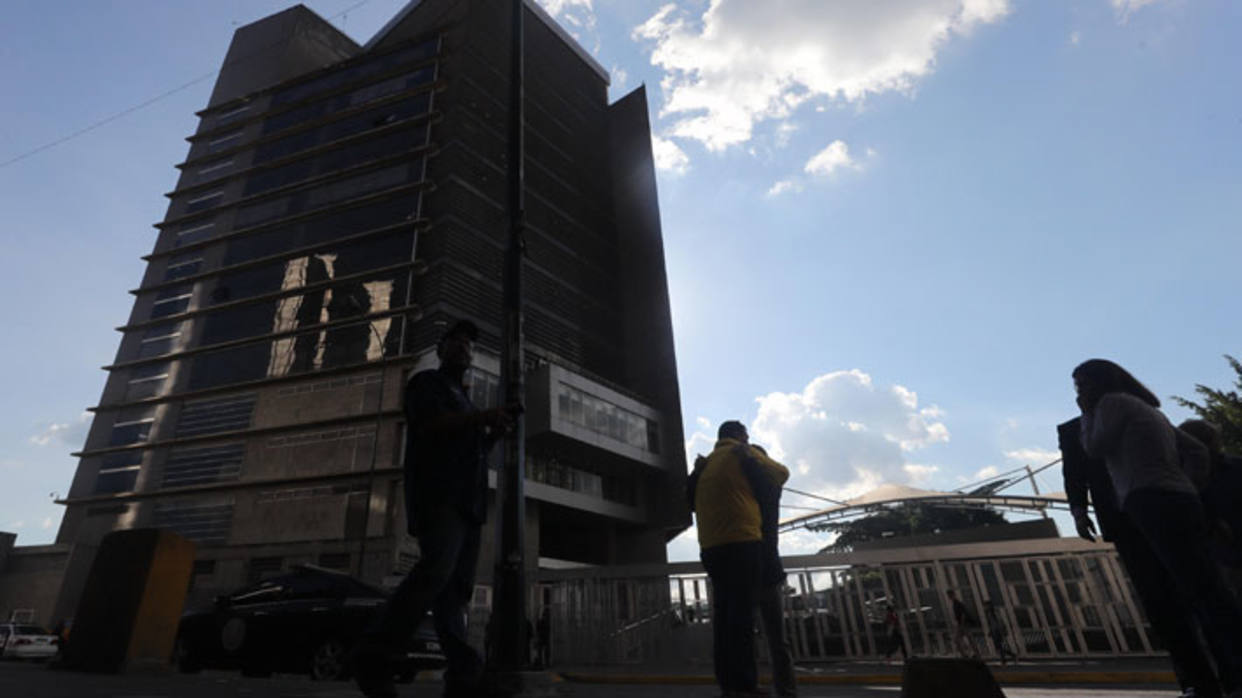
\includegraphics[width=300px]{9.jpg}%
\newline%
%
Diego Salazar y José Enrique Luongo, detenidos hace un año en Venezuela por corrupción en la petrolera Pdvsa~durante la presidencia de Hugo Chávez, permanecen recluidos en "La Tumba", donde desde entonces solo han visto 15 horas de luz solar y no han pasado aún ante un juez, informaron~a~Efe~fuentes de su entorno.%
\newline%
%
El centro de detención está bajo la sede del Servicio Bolivariano de Inteligencia (Sebin) de Plaza Venezuela en Caracas y desde el 2 de diciembre de 2017 alberga a estos dos investigados por corrupción.%
\newline%
%
Entre ellos son primos lejanos y Salazar es, a su vez, primo hermano del ex ministro de Energía y ex presidente de Pdvsa,~Rafael Ramírez, uno de los hombres más poderosos de Venezuela con Chávez y en la actualidad exiliado, sin que se conozca su paradero.%
\newline%
%
"Es un lugar tan blanco y frío como un quirófano; la asepsia es casi la de un hospital y su blancura y su brillo es el de un quirófano", relatan las fuentes.%
\newline%
%
Diego Salazar da nombre al que la Justicia venezolana llama el "grupo Salazar", un conjunto de personas perseguidas por las autoridades~y relacionadas con Ramírez, a quien supuestamente ayudaron a desviar fondos de la petrolera estatal, que presidió de 2004 a 2014.%
\newline%
%
Al menos dos de sus miembros y el que fuera número dos de Ramírez, el ex viceministro de Energía Nervis Villalobos, han sido localizados en España, y Venezuela ha pedido su extradición, pero la Justicia española, de momento, se ha opuesto a entregar a uno de ellos, el ex contable de Pdvsa José Ramón Sánchez Rodríguez, por miedo a que sea maltratado en su país.%
\newline%
%
Lo ha hecho apoyándose en documentos que aportó el abogado de Sánchez Rodríguez, Ismael Oliver, en los que se refiere a una veintena de peticiones, hasta ahora desoídas, de los abogados de Salazar y Luongo para que les dejen ver la luz del sol, les reconozcan médicos y pasen a disposición del juez, que ha solicitado tomarles declaración hasta en ocho ocasiones.%
\newline%
%
En el caso de Salazar, de 50 años, los abogados alegan que padece un trastorno bipolar y muestra pensamientos suicidas, sobre todo después de que la Justicia venezolana echara a su mujer y tres hijos de su domicilio y una de sus niñas intentara suicidarse.%
\newline%
%
"Cuando estás ahí 24 horas al día y tienes algún antecedente psiquiátrico, te altera tu estabilidad emocional", resume su entorno, que explica que su estado físico se ha deteriorado.%
\newline%
%
Salazar ha reclamado una docena de veces al juzgado y a la Fiscalía venezolana que le examine un psiquiatra y que se designe un fiscal para investigar las condiciones de su reclusión, pero no lo ha logrado.%
\newline%
%
"No ha sido trasladado e incluso se tiene conocimiento de que la policía nacional contra la corrupción se ha negado a recibir los oficios que le son dirigidos, afirmando que no está bajo su custodia", dice uno de los escritos aportado a la Justicia española.%
\newline%
%
La situación irregular de Salazar se extiende a su familia, porque~la Justicia ha quitado los pasaportes venezolano e italiano a sus tres hijos (uno de 12 años y dos gemelas de 15), reconociendo que la medida persigue prevenir la posible fuga de la madre, también imputada.%
\newline%
%
El caso de Luongo, de 64 años, es parecido. Su defensa afirma que padece demencia senil y requiere de un control neurológico constante, cosa que no se le ha facilitado en su celda.%
\newline%
%
\end{document}